\chapter{AI Component Design}
\label{chap:ai-component-design}

\section{Business Context and AI Integration}
\label{section:business_context}
\usevar{\srsTitle} tackles the complex challenge of tracking individuals across multiple camera views in environments like campuses and factories. The core task requires recognizing and associating individuals as they move between potentially non-overlapping camera fields, often amidst changing appearances, viewpoints, lighting conditions, and occlusions. This inherent complexity and real-world variability make manual tracking labor-intensive, error-prone, and difficult to address effectively with traditional rule-based programming. Artificial Intelligence is therefore central to \usevar{\srsTitle}, providing the automation necessary to significantly improve this process.

The primary AI-driven workflow resides within the system's backend processing core, designed as a service-oriented architecture. This backend, built with FastAPI, orchestrates a pipeline for retrospective analysis of recorded video feeds. Video data (pre-split into manageable sub-video segments) is fetched from cloud storage (e.g., AWS S3) and cached locally for processing. The AI pipeline involves several key steps for each frame extracted from these video segments:
\begin{enumerate}
    \item \textbf{Person Detection:} Identifying individuals within each camera frame using high-performance detection models (e.g., Faster R-CNN).
    \item \textbf{Intra-Camera Tracking:} Maintaining consistent temporary IDs for detected individuals within a single camera's view over consecutive frames, utilizing robust tracking algorithms (e.g., BotSort).
    \item \textbf{Feature Extraction for Re-ID:} Generating unique appearance embeddings (features) from detected person images using discriminative feature extraction models (e.g., CLIP).
    \item \textbf{Cross-Camera Re-Identification (Re-ID):} Matching these appearance embeddings across different camera views and time gaps to assign a persistent global identity, linking temporary tracks together. This involves managing an embedding gallery, potentially using Redis for recent embeddings and TimescaleDB for historical ones.
    \item \textbf{Spatial Mapping:} Transforming the detected location of individuals from the camera's 2D image plane onto a unified top-down map coordinate system using geometric transformation techniques (e.g., homography matrices).
\end{enumerate}
These AI components perform the essential visual analysis and identity association. Tracking metadata (bounding boxes, global IDs, map coordinates, frame timestamps) is then compiled and can be streamed to a frontend client via WebSockets for visualization, while historical data is stored in TimescaleDB. Figure \ref{fig:system_architecture} provides a high-level illustration of this system architecture and the integration points for these AI modules.
\begin{figure}[!htb] % Use !htb to suggest placement: here, top, bottom
    \centering
    \makebox[\textwidth][c]{
        \includegraphics[width=1.0\textwidth, keepaspectratio]{jubjones/architecture.jpg}
    }
    \caption{System Architecture Overview Highlighting AI Component Integration}
    \label{fig:system_architecture}
\end{figure}
\clearpage % Ensure figure placement doesn't clash excessively with text
The justification for employing AI stems from the nature of the problem itself:
\begin{itemize}
    \item \textbf{Complexity Beyond Rules:} Recognizing and matching people under diverse visual conditions involves intricate pattern recognition that surpasses the capabilities of predefined rules. AI models excel at learning these complex patterns directly from data.
    \item \textbf{Scalability Requirement:} Manually monitoring and correlating feeds from numerous cameras is impractical. AI offers an automated solution capable of handling large data volumes and multiple camera streams for retrospective analysis.
    \item \textbf{Adaptability to Dynamic Environments:} Real-world surveillance scenarios are constantly changing. AI, particularly deep learning, offers better generalization and adaptation to variations in lighting, crowds, and individual appearances compared to static algorithms.
    \item \textbf{Value Despite Imperfection:} Achieving flawless accuracy in cross-camera tracking is exceptionally difficult due to the inherent ambiguities and challenges (e.g., severe occlusions, drastic appearance changes). However, an AI system achieving high, albeit imperfect, accuracy still delivers significant value. It drastically reduces the manual workload for operators and provides a level of situational awareness unattainable through manual means or simpler systems. Even with occasional errors, such as false positive matches or missed detections, the system's ability to automatically correlate identities across most views aligns with the primary goal of enhancing operational efficiency and speeding up investigations. The objective is a substantial improvement over the baseline, accepting a trade-off where occasional inaccuracies are outweighed by the overall gains in automation and insight.
\end{itemize}

\section{Goal Hierarchy}
\label{section:goal_hierarchy}
Ensuring the AI components effectively contribute to the overall success of \usevar{\srsTitle} requires aligning goals across multiple levels. This hierarchical approach clarifies the purpose of each component and provides measurable targets for development and evaluation, moving from broad organizational objectives down to specific AI model performance.
\begin{itemize}
    \item \textbf{Organization Level Goals:}
        \begin{itemize}
            \item Enhance overall campus/factory safety and security posture.
            \item Improve operational efficiency for security and facility management teams.
            \item Optimize resource allocation (e.g., personnel deployment, space utilization).
            \item Reduce costs associated with manual surveillance monitoring and incident investigation time.
        \end{itemize}
        \textbf{Measurement:} Success at this level is measured via key performance indicators such as reduction in security incidents, faster incident resolution times, documented improvements in space utilization, and potential reduction in monitoring personnel hours.
    \item \textbf{System Level Goals (\usevar{\srsTitle}):}
        \begin{itemize}
            \item Provide accurate and continuous tracking of individuals across multiple, potentially non-overlapping, camera views from recorded footage.
            \item Maintain persistent identity of individuals even through temporary disappearances or view changes in the analyzed data.
            \item Visualize individual movement paths clearly on a unified spatial map.
            \item Enable efficient retrospective analysis of movement patterns and incidents.
            \item Offer a reliable and usable interface for target users.
        \end{itemize}
        \textbf{Measurement:} System success is assessed through end-to-end tracking accuracy metrics (e.g., overall MOTA/IDF1 on test sequences), system processing throughput for batch analysis, task completion time for key user scenarios, and user satisfaction surveys.

    \item \textbf{User Level Goals:}
        \begin{itemize}
            \item \textit{Security Officer:} Faster POI location/monitoring during investigations, efficient evidence gathering from historical data, reduced manual correlation effort. (\ref{userstory:1}, \ref{userstory:2}, \ref{userstory:5})
            \item \textit{Facility Manager:} Understanding pedestrian flow from past data, identifying bottlenecks, optimizing space. (\ref{userstory:3})
            \item \textit{Emergency Coordinator:} Rapid location finding during post-incident analysis, reviewing evacuations. (\ref{userstory:5})
            \item \textit{Analytics Specialist:} Accessing historical data for trend analysis. (\ref{userstory:4})
        \end{itemize}
        \textbf{Measurement:} User-level success is evaluated by measuring time savings for specific analytical tasks (e.g., time to locate a person's full path in historical data), task success rates, positive feedback on usability and effectiveness, and the perceived accuracy of generated movement analyses.

    \item \textbf{AI Model Level Goals:}
        \begin{itemize}
            \item \textit{Detection Model:} Achieve high precision and recall for person detection across diverse conditions in recorded video.
            \item \textit{Tracking Model:} Minimize identity switches (IDSW) and fragmentation within single cameras, achieving high MOTA and IDF1 scores on benchmark datasets.
            \item \textit{Re-Identification Model:} Generate highly discriminative appearance features, achieving high Rank-1 accuracy and mAP for cross-camera matching on benchmark datasets.
            \item \textit{Spatial Mapping Component:} Accurately transform image coordinates to map coordinates with minimal projection error using pre-supplied calibration data.
        \end{itemize}
        \textbf{Measurement:} AI model performance is quantified using standard computer vision benchmarks on relevant datasets (like the MTMMC test split), including metrics such as Average Precision (AP), Recall, MOTA, MOTP, IDF1, IDSW, Rank-1 Accuracy, mAP, CMC curves, and coordinate projection error where applicable.
\end{itemize}
To comprehensively evaluate the system and ensure it meets its objectives, a variety of data will be collected. This includes quantitative performance metrics from the AI models themselves (such as detection accuracy, tracking precision, and re-identification success rates on benchmark datasets like MTMMC), system-level operational data (like processing speed for batch tasks, error logs), and qualitative user feedback (gathered through surveys, interviews, and observation of users interacting with the system during pilot phases or usability testing). We will know if the system is doing a good job by analyzing these collected data points against the predefined success criteria outlined at each level of the goal hierarchy. Specifically, success will be indicated by strong AI model performance on technical benchmarks, efficient system operation for analytical tasks, and demonstrable improvements in user task efficiency, coupled with positive user satisfaction regarding the system's effectiveness and usability in achieving their respective goals. Continuous monitoring of these aspects will guide further development and refinement.

\section{Task Requirements Analysis Using AI Canvas}
\label{section:task_analysis_aic}
This section breaks down the core AI task of multi-camera person tracking using the AI Canvas framework to clarify requirements, inputs, outputs, and evaluation criteria.

\subsection{AI Task Requirements}
\label{subsection:ai_task_reqs_aic}
The AI components must meet the following requirements within the specified operational environment and constraints for retrospective analysis:
\begin{itemize}
    \item \textbf{Requirements (REQ):} The fundamental goals the AI must achieve.
        \begin{itemize}
            \item Accurately detect individuals in diverse video frames from multiple cameras sourced from recorded footage.
            \item Reliably track detected individuals within the field of view of a single camera over time.
            \item Correctly associate, or re-identify, the same individual when they appear across different camera views in the recorded data, potentially after time gaps or significant appearance changes.
            \item Provide the spatial location of tracked individuals within a unified coordinate system (map).
        \end{itemize}
    \item \textbf{Specifications (SPEC):} The necessary technical capabilities.
        \begin{itemize}
            \item Implement high-performance person detection capabilities suitable for surveillance footage.
            \item Employ robust tracking algorithms capable of handling short-term occlusions and maintaining identity within a single camera view.
            \item Utilize methods to generate discriminative appearance features from person images, enabling effective re-identification.
            \item Apply appropriate similarity metrics to compare appearance features for matching individuals across views.
            \item Incorporate techniques for transforming image coordinates to a common spatial map reference frame using provided calibration data.
        \end{itemize}
    \item \textbf{Environment (ENV):} The operational context, including assumptions and limitations.
        \begin{itemize}
            \item Input consists of sequential image frames extracted from recorded video segments from a network of potentially non-overlapping cameras operating in real-world campus or factory settings.
            \item The system is designed to operate under typical environmental challenges found in such recordings, but performance relies on certain assumptions and is subject to limitations:
                \begin{itemize}
                    \item \textbf{Appearance Consistency:} Assumes individuals do not drastically change their core appearance (e.g., changing distinct clothing) between consecutive camera views within the tracking period relevant to the analysis. Re-ID relies heavily on visual similarity.
                    \item \textbf{Lighting Variations:} While robust to moderate lighting changes, extreme variations present in the recordings can significantly degrade detection and Re-ID performance.
                    \item \textbf{Occlusion Handling:} Tolerant to short-term, partial occlusions. However, prolonged periods where an individual is completely hidden from all camera views in the footage may lead to track fragmentation or loss.
                    \item \textbf{Crowding:} Performance may degrade in extremely dense crowds where individuals are heavily occluded for extended durations.
                    \item \textbf{Viewpoint Changes:} Designed to handle viewpoint variations, but extreme differences can impact feature distinctiveness for Re-ID.
                \end{itemize}
            \item Processing occurs within the backend system, requiring adequate computational resources (potentially including GPUs) to handle the batch processing workload.
        \end{itemize}
\end{itemize}

\subsection{AI Canvas Development}
\label{subsection:ai_canvas_dev_aic}
Applying the AI Canvas framework helps to structure the analysis of the primary AI task: assigning a consistent global identity across multiple camera views from recorded footage.
Figure \ref{fig:ai_canvas} illustrates this.
\begin{figure}[!htb]
    \centering
    \makebox[\textwidth][c]{
        \includegraphics[width=1.0\textwidth, keepaspectratio]{jubjones/ai_canvas.jpg}
    }
    \caption{AI Canvas for Multi-Camera Person Tracking}
    \label{fig:ai_canvas}
\end{figure}
\clearpage
\begin{itemize}
    \item \textbf{Task/Decision Examined:} The core task is to determine if a person detected in one camera view at a certain time is the same individual as a person detected in another (or the same) camera view at a later time within the analyzed video data. This involves combining detection, tracking, and re-identification.
    \item \textbf{Prediction:} The key uncertainty the AI needs to resolve is: "Given appearance features (embedding) extracted from track A in camera X and features from track B in camera Y, what is the probability that A and B represent the same unique individual?"

    \item \textbf{Judgment:} Evaluating the correctness of the prediction involves considering the payoffs:
        \begin{itemize}
            \item \textit{Correct Match (True Positive):} Enables seamless tracking, accurate path reconstruction. Payoff: High system utility, user trust in analytical results.
            \item \textit{Incorrect Match (False Positive - Mismatch):} Assigns the same ID to different people. Payoff: Negative - Corrupts historical data, misleads users, significantly erodes trust.
            \item \textit{Missed Match (False Negative):} Fails to link the same person across views. Payoff: Negative - Creates fragmented tracks, reduces system effectiveness for analysis, may require manual reconciliation if possible.
        \end{itemize}
        Minimizing false positive mismatches is often critical for maintaining data integrity and user confidence, even if it leads to slightly more missed matches (fragmented tracks).

    \item \textbf{Action:} Based on the prediction (similarity score and threshold):
        \begin{itemize}
            \item If similarity is high (above threshold): Associate the tracks by assigning the existing GlobalPersonID.
            \item If similarity is low (below threshold): Treat as a different individual, assign a new GlobalPersonID.
        \end{itemize}

    \item \textbf{Outcome:} Performance is measured using standard metrics on benchmark datasets:
        \begin{itemize}
            \item \textit{Primary Tracking Metrics:} IDF1 Score (identity preservation), MOTA (overall tracking accuracy).
            \item \textit{Re-ID Specific Metrics:} Rank-1 Accuracy, mean Average Precision (mAP).
            \item \textit{System-Level Metrics:} Reduction in manual effort for historical analysis, time-to-completion for finding a person's full path in recorded data.
        \end{itemize}

    \item \textbf{Training:} To train the AI components (especially detection and Re-ID models):
        \begin{itemize}
            \item Need large datasets of annotated video sequences (like MTMMC train/val splits).
            \item Annotations must include bounding boxes per frame and consistent person IDs *within* each camera view.
            \item Crucially, need ground truth *global identities* linking person appearances across different cameras to train and evaluate the Re-ID model effectively.
        \end{itemize}

    \item \textbf{Input (for Prediction during retrospective analysis):} Once trained, the system needs:
        \begin{itemize}
            \item Incoming video frames extracted from sub-video segments fetched from cloud storage (e.g., S3).
            \item Bounding boxes generated by the person detector.
            \item Appearance embeddings generated by the Re-ID feature extractor for relevant detections/tracks.
            \item Camera calibration data (e.g., homography matrices) for spatial mapping, specific to each camera.
        \end{itemize}

    \item \textbf{Feedback:} Improving the AI relies on analyzing outcomes:
        \begin{itemize}
            \item Use evaluation metrics (MOTA, IDF1, mAP, etc.) on test data to identify weaknesses.
            \item Tune hyperparameters (e.g., Re-ID matching threshold, detection confidence) based on performance trade-offs.
            \item Analyze failure cases to inform retraining strategies or data augmentation techniques.
        \end{itemize}

    \item \textbf{Impact on Workflow:}
        \begin{itemize}
            \item Automates the time-consuming and error-prone task of manually correlating identities across camera feeds in historical footage.
            \item Enables visualization of movement paths across the entire monitored area from past recordings.
            \item Frees up security/facility personnel to focus on higher-level tasks like incident investigation, trend analysis, and strategic planning rather than low-level video review.
            \item Requires user training on the interface for retrospective analysis and building trust in the AI's associations. It augments staff capabilities for investigation and analysis.
        \end{itemize}
\end{itemize}

Figure \ref{fig:ml_canvas} illustrates the comprehensive ML Canvas design specifically tailored for the Intelligent Multi-Camera Person Tracking and Analytics System. This canvas provides a detailed blueprint for the ML components, building upon the general AI task analysis.

\begin{figure}[!htb]
    \centering
    \makebox[\textwidth][c]{
        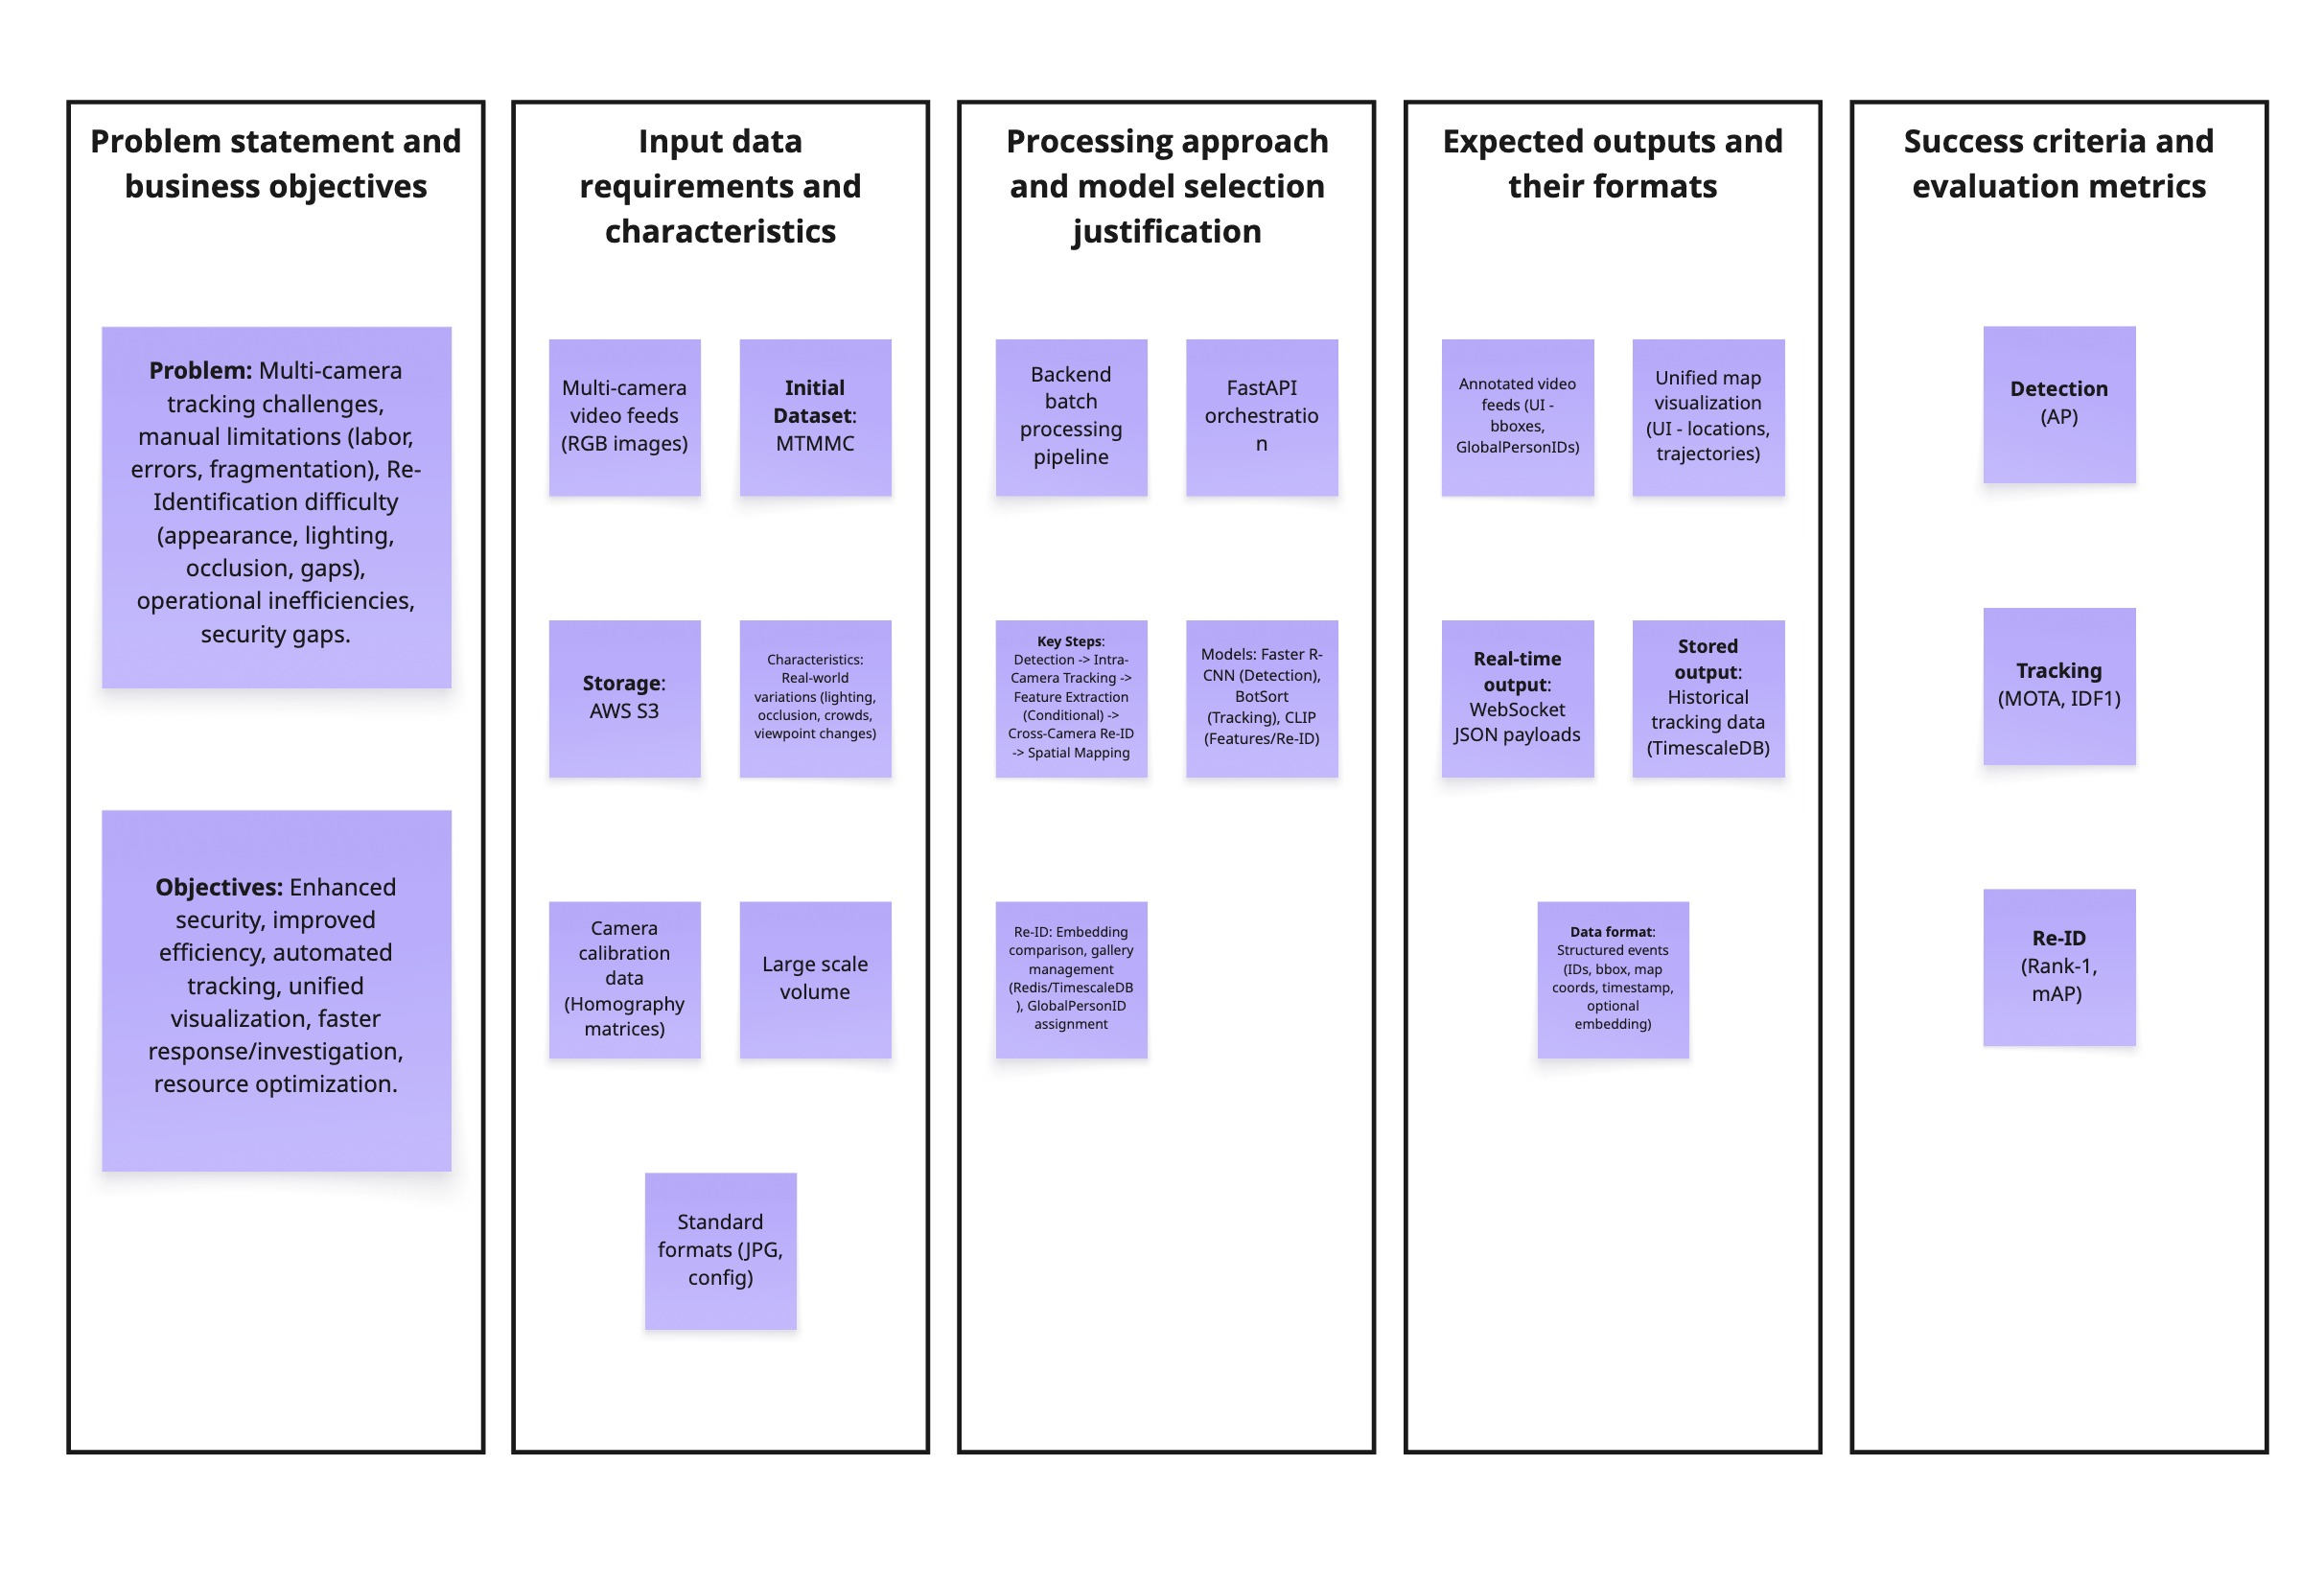
\includegraphics[width=1.0\textwidth, keepaspectratio]{jubjones/ml_canvas.jpg}
    }
    \caption{ML Canvas for Intelligent Multi-Camera Person Tracking and Analytics System}
    \label{fig:ml_canvas}
\end{figure}
\clearpage
\begin{itemize}
    \item \textbf{Problem Statement \& Business Objectives (ML Canvas):}
        The system directly addresses the significant challenges security and facility personnel face in tracking individuals across complex, multi-camera environments using recorded data. It tackles the limitations of manual review—its labor intensity, error propensity, and fragmented views—and the core technical hurdle of maintaining consistent identity (Re-Identification) despite variations in appearance, lighting, occlusions, and camera viewpoints present in historical footage. The overarching business objectives are to enhance safety through better post-incident analysis, improve operational efficiency by automating tracking in recorded data, provide unified spatial visualization of movement, reduce incident investigation time, and optimize resource allocation based on analytics from past events.

    \item \textbf{Input Data Requirements (ML Canvas):}
        The necessary components for the system primarily involve recorded RGB video feeds (pre-split into sub-videos) or image sequences from multiple cameras, initially using datasets like MTMMC stored on cloud storage (e.g., AWS S3). These inputs encapsulate real-world challenges. Pre-calculated camera calibration data (Homography matrices) are essential inputs for spatial mapping.

    \item \textbf{Processing Approach \& Model Selection (ML Canvas):}
        Central to the design is a backend-driven batch processing pipeline orchestrated by FastAPI. This pipeline integrates key AI steps in sequence:
        \begin{enumerate}[label=(\Alph*)]
            \item Person Detection, utilizing models like Faster R-CNN for robust object localization.
            \item Intra-Camera Tracking, employing algorithms like BotSort (potentially via BoxMOT) to maintain temporary IDs within single camera views.
            \item Conditional Feature Extraction for Re-ID, using models like CLIP (potentially via BoxMOT) to generate discriminative embeddings.
            \item Cross-Camera Re-Identification, which compares embeddings against a gallery (managed via Redis for recent/active data and TimescaleDB for historical data) to assign persistent GlobalPersonIDs.
            \item Spatial Mapping, applying input homography matrices via libraries like OpenCV to project detected locations onto a unified map.
        \end{enumerate}
        The justifications for model choices emphasize accuracy, robustness, and efficiency for retrospective analysis.

    \item \textbf{Expected Outputs (ML Canvas):}
        The system's outputs encompass both user-facing visualizations and stored data for analysis.
        \begin{itemize}
            \item \textit{For the UI (from backend metadata):} Annotated video feeds (client-side rendering of bounding boxes and GlobalPersonIDs based on WebSocket metadata) alongside a unified map interface showing current locations and historical paths.
            \item \textit{For historical analysis:} Structured tracking events (timestamp, IDs, coordinates, optional embeddings) stored in a TimescaleDB database.
        \end{itemize}

    \item \textbf{Success Criteria \& Evaluation Metrics (ML Canvas):}
        A dual approach to measuring performance is outlined:
        \begin{itemize}
            \item \textit{AI Model-Level Metrics (Offline Evaluation):} Specific metrics such as AP (Average Precision), MOTA (Multiple Object Tracking Accuracy), IDF1 (ID F1-Score), Rank-1 accuracy, and mAP (mean Average Precision) using dedicated test sets from datasets like MTMMC.
            \item \textit{System and Business-Level Metrics (Operational Assessment):} Critical indicators including efficiency gains in analytical tasks, reduction in incident investigation response time, user satisfaction levels, task completion rates for key scenarios using the system, and overall system reliability during batch processing.
        \end{itemize}
\end{itemize}
This detailed ML Canvas provides a comprehensive blueprint for the development and evaluation of this intelligent surveillance analysis system.

\subsection{(Optional) Innovation}
\label{subsection:innovation_aic}
While \usevar{\srsTitle} leverages established AI techniques for tasks like detection, tracking, and re-identification, its core innovation lies in the effective integration and adaptation of these methods into a cohesive backend system designed for retrospective analysis of multi-camera footage from complex real-world environments. The system architecture, emphasizing modularity with a service-oriented approach using FastAPI, scalable data handling from cloud storage (S3), and efficient data management (Redis, TimescaleDB), allows for robust processing of recorded data. The focus on providing actionable metadata via WebSockets for rich client-side visualization, combined with persistent storage for in-depth historical analysis, addresses the practical needs of surveillance review and investigation where maintaining identity consistently across non-overlapping views with temporal gaps is paramount.

\section{AI Model Development and Evaluation}
\label{section:ai_model_dev_eval_new}
This section outlines the strategy for developing, training, and evaluating the core AI models that underpin the \usevar{\srsTitle} system, focusing on the person detection component as a critical foundation.

\subsection{Model Development and Training Strategy}
\label{subsection:model_dev_train_strat_new}
The primary AI model for person detection, such as Faster R-CNN with a ResNet-50 backbone and Feature Pyramid Network (FPN), was developed using the PyTorch deep learning framework. The development process prioritized robustness and accuracy for surveillance footage analysis.
Key aspects of the strategy include:
\begin{itemize}
    \item \textbf{Dataset Utilization:} The MTMMC dataset served as the primary data source for training and fine-tuning. This dataset's diversity in campus and factory environments, lighting conditions, and occlusion levels provides a realistic foundation for developing models intended for real-world scenarios.
    \item \textbf{Transfer Learning:} To leverage knowledge from broader datasets and accelerate convergence, models were initialized with pre-trained weights (e.g., from ImageNet). The classification head of the detection model was then modified and fine-tuned to specifically address the 'person' class (and background) relevant to the system's objectives.
    \item \textbf{Data Preprocessing:} A standardized preprocessing pipeline was established. This included image resizing to a consistent input dimension for the model, color space conversion (e.g., BGR to RGB), normalization using established statistics (e.g., ImageNet mean and standard deviation), and conversion to tensor formats suitable for PyTorch. Data augmentation techniques, such as random horizontal flipping, were applied during training to enhance model generalization.
    \item \textbf{Experiment Management:} A systematic approach to tracking experiments, model configurations, hyperparameters, and performance metrics was employed, often facilitated by tools designed for experiment management (e.g., MLflow). This allowed for methodical comparison of different training runs and model variants.
\end{itemize}
This structured approach ensured that the model development lifecycle was organized, reproducible, and geared towards optimizing performance on the target task.

\subsection{Testing and Validation Approach}
\label{subsection:model_test_validate_new}
Rigorous testing and validation were integral to ensure the reliability and effectiveness of the AI models. The approach encompassed several layers:
\begin{itemize}
    \item \textbf{Quantitative Evaluation on Benchmark Data:} The primary method for assessing model performance involved testing against a dedicated validation split of the MTMMC dataset. Standard COCO-style metrics were employed, particularly mean Average Precision (mAP) at various Intersection over Union (IoU) thresholds (e.g., mAP@.50, mAP@[.50:.95]). The Average Precision (AP) specifically for the 'person' class served as a critical performance indicator.
    \item \textbf{Comparative Model Analysis:} To select the most suitable baseline detection model for the system, a comparative analysis of different candidate architectures was performed. This involved training and evaluating several models (e.g., Faster R-CNN, RT-DETR variants, YOLO variants) under consistent conditions. Performance was assessed based on quantitative accuracy metrics (like mAP), inference speed (Frames Per Second - FPS), and qualitative observations of detection stability on representative video data. The process of comparing models, including visualization of performance trade-offs (as conceptually illustrated in Figure \ref{fig:mlflow_comparison_1}) and tabular summaries of key metrics (conceptually represented by Figure \ref{fig:mlflow_comparison_2}), guided the selection.
    \item \textbf{Unit Testing of Core Components:} Key software components within the training and evaluation pipeline, such as dataset loading mechanisms, annotation parsing utilities, metric calculation functions, and model instantiation logic, were subjected to unit tests. This helped ensure the correctness and reliability of the underlying codebase supporting the AI model lifecycle.
    \item \textbf{Fairness Considerations:} An initial analysis of potential biases in the training data (MTMMC) and model behavior was considered. This involved identifying potential sources of bias (e.g., demographic imbalances, environmental variations) and discussing conceptual mitigation strategies (e.g., targeted data augmentation, fairness-aware training if feasible, transparency). While a full quantitative fairness audit requires specific demographic ground truth often unavailable, this proactive consideration is crucial for responsible AI development.
\end{itemize}

\begin{figure}[!htb]
    \centering
    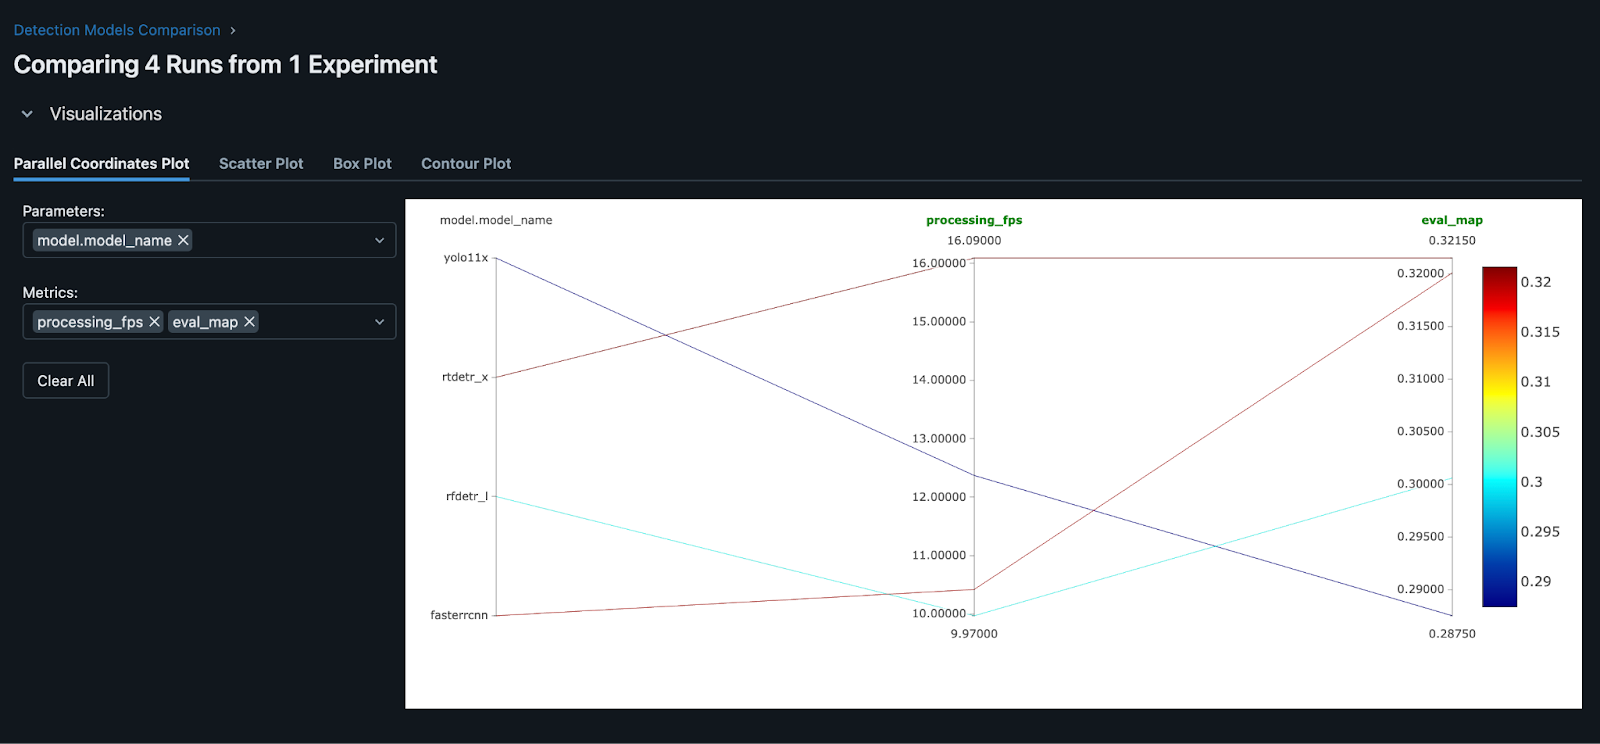
\includegraphics[width=1.0\textwidth,keepaspectratio]{jubjones/mlflow_comparison_1.png}
    \caption{Conceptual Illustration: Chart Comparing Performance Metrics of Different Detection Models}
    \label{fig:mlflow_comparison_1}
\end{figure}

\begin{figure}[!htb]
    \centering
    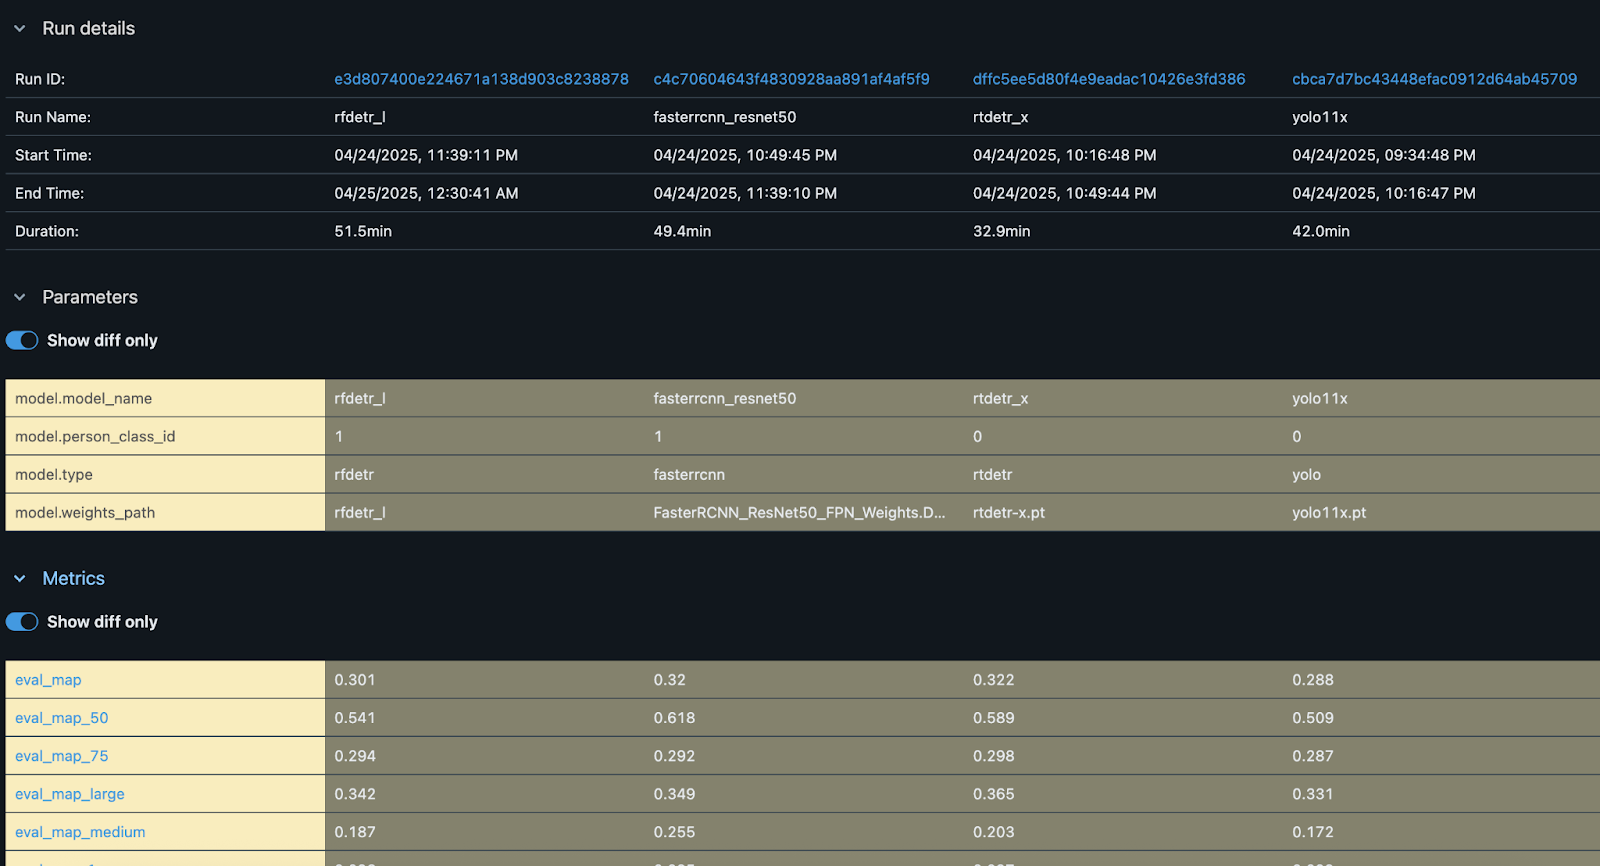
\includegraphics[width=1.0\textwidth,keepaspectratio]{jubjones/mlflow_comparison_2.png}
    \caption{Conceptual Illustration: Table Summarizing Key Performance Metrics for Model Comparison}
    \label{fig:mlflow_comparison_2}
\end{figure}
\clearpage

\subsection{Performance Results and Justification}
\label{subsection:model_perf_justify_new}
The comparative analysis of various person detection models, aided by experiment tracking tools, led to the selection of Faster R-CNN as the baseline architecture for the \usevar{\srsTitle} system. While other models, such as certain RT-DETR variants, demonstrated strengths in specific areas like overall mAP or inference speed, Faster R-CNN presented a compelling balance of characteristics crucial for the system's application in retrospective surveillance analysis.

Key performance observations and the justification for selecting Faster R-CNN include:
\begin{itemize}
    \item \textbf{Strong Performance on Medium-Sized Objects:} Faster R-CNN exhibited notably good performance in detecting medium-sized persons, a common scenario in real-world surveillance footage where individuals are neither very close to the camera nor extremely distant. This capability is critical for reliable detection across typical operational distances.
    \item \textbf{High Recall / Detection Count:} Compared to some alternatives, Faster R-CNN often yielded a higher total number of person detections on the evaluation dataset. This suggests superior recall, which is vital in a tracking system to minimize missed detections (false negatives). A missed detection can lead to a complete loss of a track, which is generally more detrimental than a lower precision if false positives can be managed.
    \item \textbf{Acceptable Processing Speed:} While not always the fastest model in terms of raw FPS, Faster R-CNN's processing speed was deemed acceptable for the backend batch processing pipeline envisioned for retrospective analysis. The system is not primarily designed for hard real-time, low-latency applications.
    \item \textbf{Qualitative Stability:} During initial practical tests on video sequences from the dataset, Faster R-CNN generally exhibited good stability, with fewer observed issues related to Non-Maximal Suppression (NMS) resulting in multiple redundant bounding boxes for the same person, compared to some other evaluated models.
\end{itemize}

\subsection{Demonstration on Representative Data (Model Explainability)}
\label{subsection:model_demo_explain_new}
To build trust and enable diagnostics, techniques were employed to understand and explain the behavior of the selected person detection model (Faster R-CNN).

\textbf{Visual Explanation of Model Focus:}
Gradient-weighted Class Activation Mapping (Grad-CAM) was utilized to generate visual heatmaps. These heatmaps highlight the regions in an input image that were most influential in the model's decision to classify an area as containing a 'person'. Figure \ref{fig:gradcam_example1} shows such a visualization for an image representative of a factory scene. The heatmap often strongly highlights relevant body parts like the torso and upper legs, aligning well with the subject's silhouette and indicating that the model learned to focus on pertinent visual features for its high-confidence detection. Similar interpretability was observed for campus scenes. For instance, Figure \ref{fig:gradcam_example2} and Figure \ref{fig:gradcam_example3} depict Grad-CAM outputs for persons detected in different campus environments. Even for smaller or more distant individuals, the heatmaps tend to concentrate on the upper body or head regions, demonstrating the model's ability to identify key features contributing to high-confidence scores. These visualizations confirm that the model generally behaves as expected by focusing on semantically relevant parts of a person.

\begin{figure}[!htb]
    \centering
    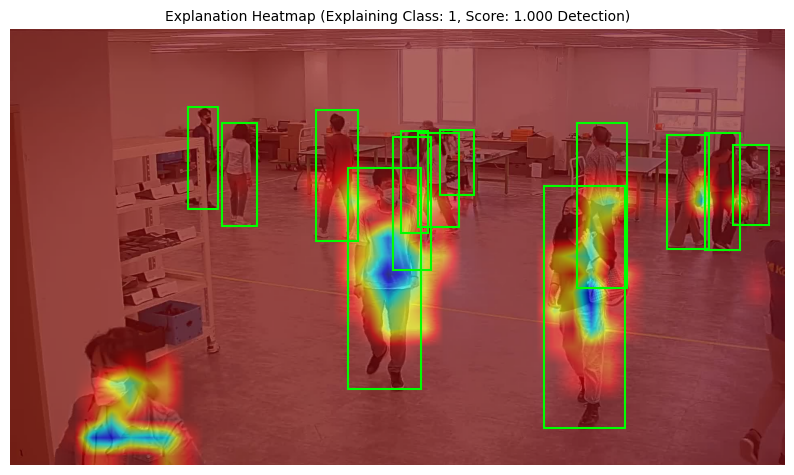
\includegraphics[width=1.0\textwidth,keepaspectratio]{jubjones/s10_c09_000000_explain_gradcam_det1_score1.00.png}
    \caption{Grad-CAM Visualization for a Person Detected in a Factory Scene Image}
    \label{fig:gradcam_example1}
\end{figure}

\begin{figure}[!htb]
    \centering
    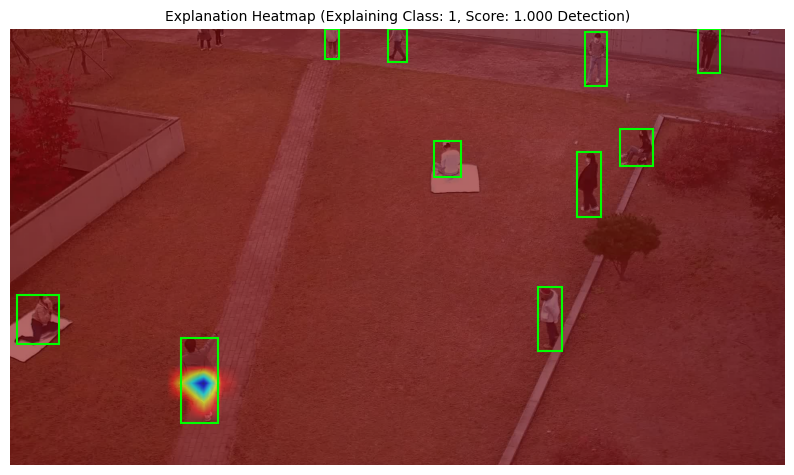
\includegraphics[width=1.0\textwidth,keepaspectratio]{jubjones/s47_c02_000000_explain_gradcam_det1_score1.00.png}
    \caption{Grad-CAM Visualization for a Person Detected in a Campus Scene Image (View 1)}
    \label{fig:gradcam_example2}
\end{figure}

\begin{figure}[!htb]
    \centering
    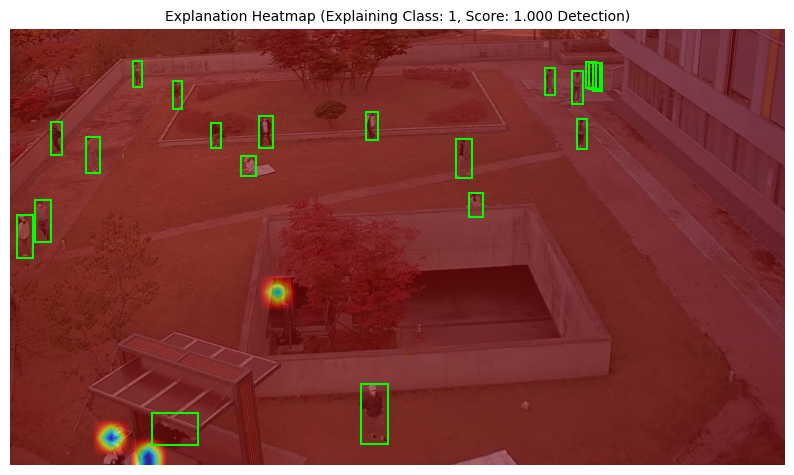
\includegraphics[width=1.0\textwidth,keepaspectratio]{jubjones/s47_c03_000000_explain_gradcam_det1_score1.00.png}
    \caption{Grad-CAM Visualization for a Person Detected in a Campus Scene Image (View 2)}
    \label{fig:gradcam_example3}
\end{figure}
\clearpage

\textbf{Textual Reasoning for Predictions:}
Beyond visual heatmaps, a mechanism was designed to generate human-understandable textual reasoning for individual predictions. This reasoning typically combines the model's quantitative output (confidence score) with a qualitative interpretation and a reference to the visual explanation. For example, for a high-confidence detection, the system might generate reasoning such as:
"Detected object classified as 'person' with a high confidence score (e.g., 0.99 or higher). This suggests the model found strong visual evidence matching features learned for the 'person' class. The associated visual explanation (e.g., Grad-CAM focus) highlights the specific image regions that most influenced this classification decision. Reviewing this visual explanation can provide further insight into which parts of the object (e.g., head, torso) contributed most to the prediction."
This approach provides a practical level of interpretability, allowing users to understand the basis of individual detection decisions by linking the model's confidence to visual evidence of its focus.
These demonstrations of model explainability serve as valuable tools for verifying expected model behavior, debugging potential issues where the model might focus on irrelevant features, and ultimately fostering greater trust in the AI system's outputs.

\section{User Experience Design with AI}
\label{section:ux_design} % This section remains untouched as per request

\begin{figure}[H]
    \centering
    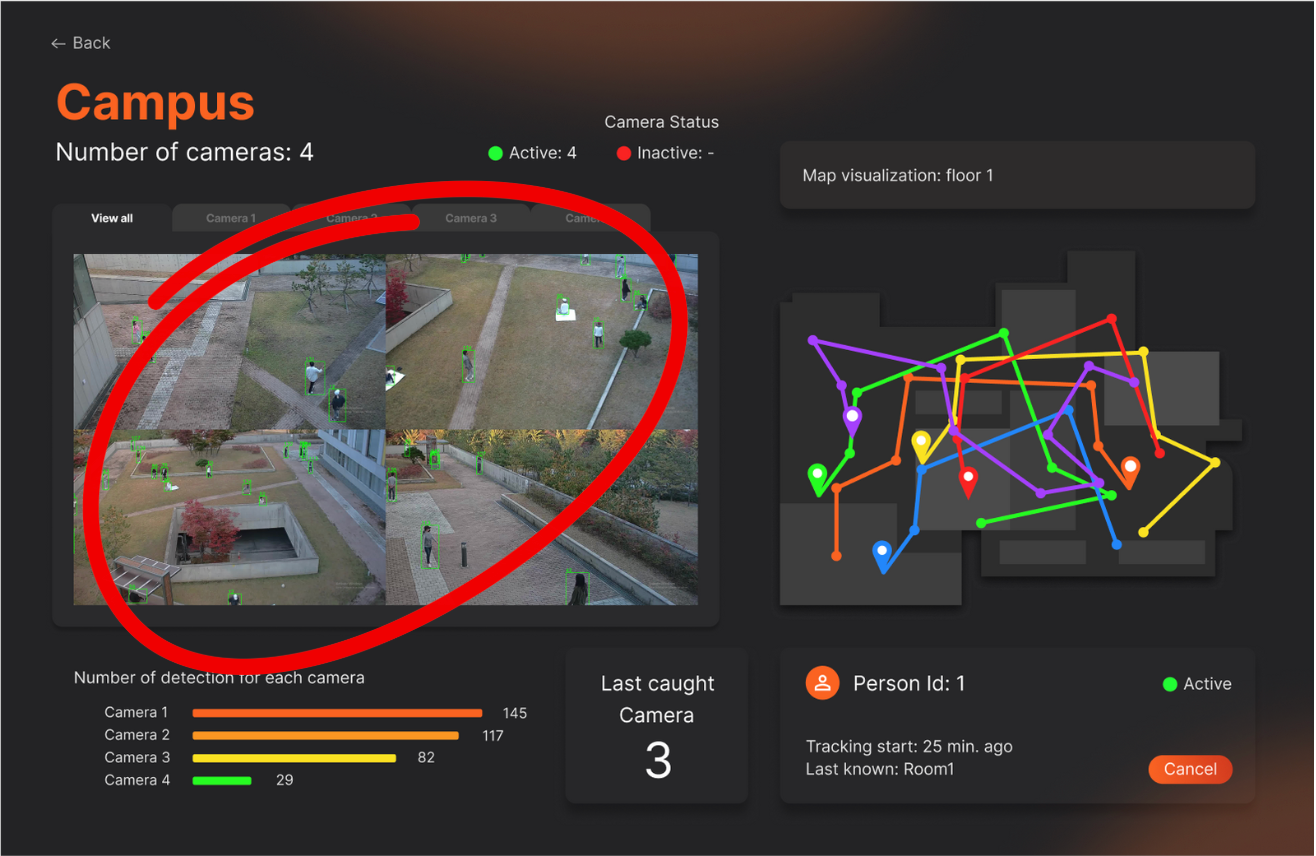
\includegraphics[width=1.0\textwidth,keepaspectratio]{assets/jubjones/ai_mockup_bbox.png}
    \caption{AI-Annotated Multi-Camera View with Person Detection.}
    \label{fig:ai_mockup_bbox}
\end{figure}

The system leverages Artificial Intelligence primarily through an Annotate interaction style to enhance the user's ability to monitor and analyze activity across multiple camera views. In this specific mockup, the AI processes the video streams from each active camera to perform person detection.
When the AI identifies a person within a camera's field of view, it annotates the visual feed by drawing a bounding box (seen as green rectangles around individuals in the composite camera display) around that person. This direct visual annotation serves multiple purposes: it immediately draws the operator's attention to the presence and specific location of individuals, helps in quickly assessing the number of people in an area, and provides a clear visual marker for each detected person. By automatically highlighting these individuals, the AI significantly reduces the cognitive load on the human operator, who no longer needs to manually scan complex scenes. These bounding boxes are fundamental AI-generated annotations that support rapid visual assessment and are a foundational element for more complex tasks like person tracking and re-identification across different cameras, which are also hinted at by the map visualization and person ID information on the right side of the interface.

\begin{figure}[!htb]
    \centering
    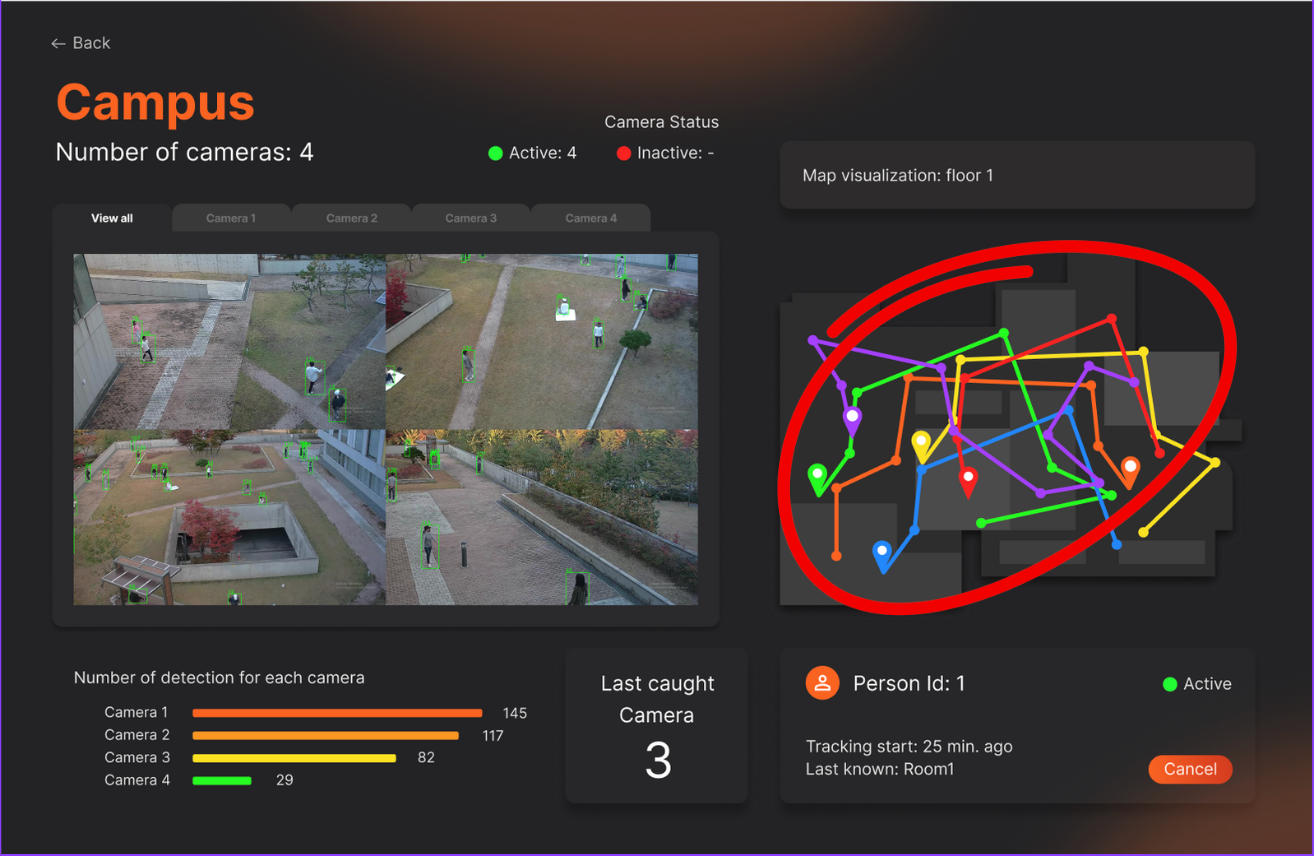
\includegraphics[width=1.0\textwidth,keepaspectratio]{assets/jubjones/ai_mockup_map.png}
    \caption{AI-Generated Trajectory Map for Multi-Person Tracking.}
    \label{fig:ai_mockup_map}
\end{figure}

The system utilizes Artificial Intelligence in an Annotate interaction style to provide users with a comprehensive spatial understanding of movement patterns within the monitored area, as depicted in the map visualization. The AI is responsible for several complex tasks that culminate in this annotated map display.
Firstly, AI models detect individuals in various camera feeds (as seen on the left). Crucially, the AI then performs cross-camera re-identification, assigning a persistent global ID to each individual and tracking them as they move between different camera views, even if those views don't overlap or if there are temporal gaps. Simultaneously, the AI uses homography or other spatial mapping techniques to transform the 2D pixel coordinates of a detected person in a camera image into corresponding coordinates on a unified 2D floor plan or map of the environment.
The map display itself is an AI-driven annotation. The lines and markers on the map are not manually drawn but are generated by the AI, representing the historical and current paths of tracked individuals. Each distinct color typically corresponds to a unique global person ID, allowing operators to visually differentiate and follow the movements of multiple people simultaneously. The location markers (pins) indicate the last known positions or significant points along these paths. This annotated map provides powerful insights into pedestrian flow, area usage, and individual trajectories, all derived from the AI's continuous processing and interpretation of multi-camera surveillance data. It transforms raw video into a spatially coherent and easily digestible overview of activity.

\begin{figure}[H]
    \centering
    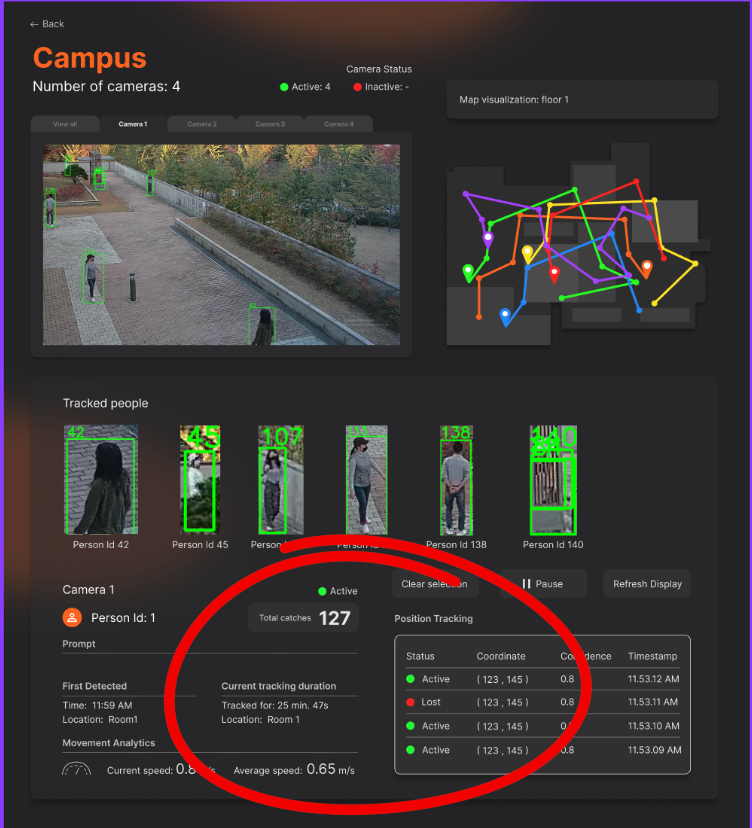
\includegraphics[width=1.0\textwidth,keepaspectratio]{assets/jubjones/ai_mockup_data.png}
    \caption{Detailed AI-Annotated Tracking Information and Movement Analytics.}
    \label{fig:ai_mockup_data}
\end{figure}

The system employs Artificial Intelligence in an Annotate interaction style to provide users with detailed, actionable insights into the behavior and history of tracked individuals, as shown in the focused panel for "Person Id: 1". This detailed view is a direct result of the AI's continuous processing and analysis of surveillance data.
The AI is responsible for initially detecting the person in a camera feed, assigning them a unique ID (Person Id: 1), and then persistently tracking their movements across time and potentially across different cameras. The "Position Tracking" table is populated by AI-derived annotations:
\begin{itemize}
    \item   \textbf{Status (Active/Lost):} The AI determines if the person is currently visible or if their track has been temporarily lost.
    \item   \textbf{Coordinate:} The AI calculates the person's location (likely map coordinates derived via homography from camera views).
    \item   \textbf{Confidence:} The AI provides a confidence score for its detection and tracking at each point in time.
    \item   \textbf{Timestamp:} Each recorded state is timestamped, allowing for a chronological review of the person's movements. 
\end{itemize}
Furthermore, the "Movement Analytics" section, displaying "Current speed" and "Average speed," is also an AI-driven annotation. The AI calculates these metrics based on the changes in the person's position over time. Information like "First Detected," "Current tracking duration," and "Location" are all data points collated and maintained by the AI's tracking algorithms.
In essence, the AI transforms raw video data into a structured, quantitative, and qualitative summary for each tracked person. This annotated information allows operators to quickly understand a person's history, assess their current state, and gain insights into their movement patterns without needing to manually review hours of footage or perform complex calculations. The AI annotates the interface with this rich data, empowering the user with a deeper understanding of the events unfolding in the monitored environment.

\section{Deployment Strategy}
\label{section:deployment_aic} % Renumbered section

\subsection{Deployment Plan}
\label{subsection:deployment_plan_aic}
\begin{itemize}
    \item \textbf{Deployment Location:}
        The AI components (e.g., person detection using Faster R-CNN, intra-camera tracking with BotSort, Re-ID feature extraction with CLIP) are integrated within the system's core \textbf{Backend} service. This Backend service, built with FastAPI, along with the entire system infrastructure (Frontend server, databases, caching, reverse proxy), is designed to be deployed in a \textbf{Cloud} environment. This leverages cloud scalability for computational resources and centralized data storage.

    \item \textbf{AI Communication with System Components:}
        The AI models run embedded within the Python-based FastAPI Backend process. Communication occurs as follows:
        \begin{itemize}
            \item \textbf{Internal Calls:} The main FastAPI application logic directly invokes the AI models for detection, tracking, feature extraction, and homography transformations using standard Python function calls.
            \item \textbf{Backend to Data Storage/Cache:} The Backend interacts with Redis (for caching Re-ID embeddings/gallery) and TimescaleDB/PostgreSQL (for storing historical tracking events and persistent embeddings) through database client libraries. It fetches video segments from cloud storage (e.g., AWS S3) and caches them locally for processing.
            \item \textbf{Backend to Frontend (Real-time Metadata):} Processed tracking metadata (bounding boxes, global IDs, map coordinates, frame timestamps) are pushed from the FastAPI Backend to the React Frontend using \textbf{WebSocket} connections. This enables real-time updates for client-side visualization overlays on video playback. The video stream itself is fetched by the client directly (e.g., from S3).
            \item \textbf{Frontend to Backend (Control/Queries):} User interactions (e.g., initiating analysis tasks, requesting historical data) are sent from the React Frontend to the FastAPI Backend via \textbf{RESTful APIs}. External communication passes through a reverse proxy like Nginx.
        \end{itemize}

    \item \textbf{Tools and Frameworks Used:}
        The deployment relies on the following key technologies:
        \begin{itemize}
            \item \textit{Containerization \& Orchestration:} \textbf{Docker} for containerizing all services.  \textbf{Docker Compose} for orchestration.
            \item \textit{Backend Framework:} \textbf{FastAPI} for REST APIs, WebSocket handling, and orchestrating the AI processing pipeline.
            \item \textit{AI Models \& Libraries:} \textbf{PyTorch} as the deep learning framework. Specific models like \textbf{Faster R-CNN} (detection), \textbf{BotSort} (tracking), \textbf{CLIP} (Re-ID feature extraction). Libraries like \textbf{BoxMOT} may be used to integrate these. \textbf{OpenCV} for video processing and image manipulation.
            \item \textit{Frontend Framework:} \textbf{React} for the user interface.
            \item \textit{Data Storage \& Caching:} Cloud storage like \textbf{AWS S3} for video segments. \textbf{Redis} for caching. \textbf{TimescaleDB} for historical tracking data and embeddings.
            \item \textit{Reverse Proxy:} \textbf{Nginx}.
            \item \textit{Monitoring \& Logging:} Tools like Prometheus, Loki, Grafana.
        \end{itemize}

    \item \textbf{System Qualities (Reliability, Security, Maintainability, Scalability):}
        The deployment strategy addresses system qualities as follows:
        \begin{itemize}
            \item \textit{Reliability:} Orchestration tools provide container health management and restarts. Monitoring tools offer visibility.
            \item \textit{Security:} Nginx acts as a gateway for security measures (HTTPS, etc.). Containerization provides isolation. Proper cloud security configurations (IAM roles, network policies) are essential.
            \item \textit{Maintainability:} Docker ensures consistent environments. Modular backend services and clear API definitions aid management. Centralized logging/metrics simplify troubleshooting.
            \item \textit{Scalability:} Cloud deployment allows resource scaling. Stateless FastAPI backend instances can be scaled horizontally. Databases and caches can be scaled using cloud services or native features. The processing pipeline is designed for batch analysis of pre-split video segments.
        \end{itemize}
\end{itemize}

\subsection{Proof of Concept (Service Demonstration)}
\label{subsection:poc_service_demo_new}
The Proof of Concept (PoC) for the \usevar{\srsTitle} system focused on demonstrating the end-to-end functionality of the AI-driven backend service, particularly its capability to process video data and stream tracking metadata for retrospective analysis.

\begin{figure}[!htb]
    \centering
    \makebox[\textwidth][c]{
        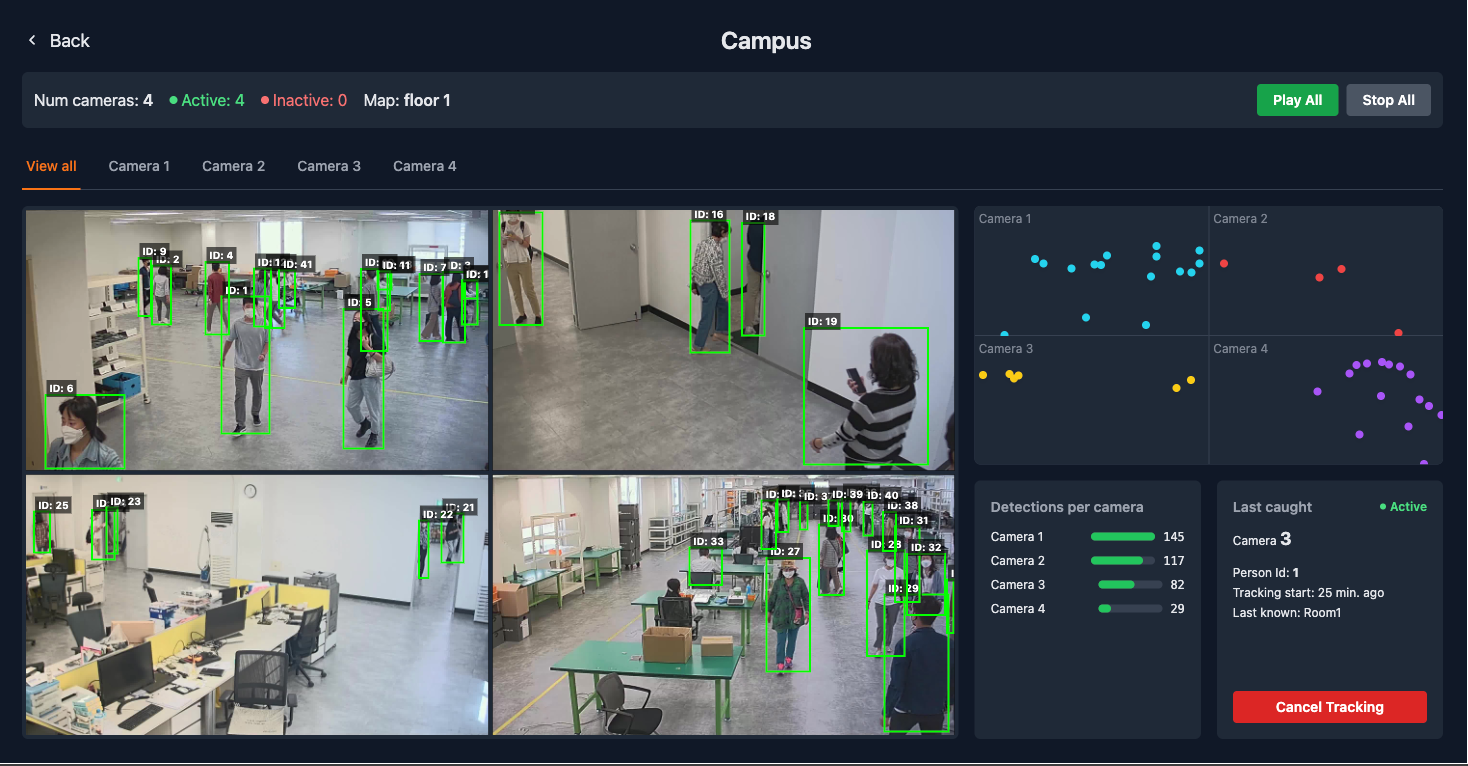
\includegraphics[width=1.0\textwidth, keepaspectratio]{jubjones/frontend_poc.png}
    }
    \caption{Frontend Proof of Concept}
    \label{fig:fontend_poc}
\end{figure}

The PoC involved the following key steps:

\begin{enumerate}
    \item \textbf{Backend Deployment:} The backend application, containerized using Docker and orchestrated with Docker Compose (including dependencies like Redis and TimescaleDB), was started. This made the system's REST APIs and WebSocket endpoint accessible.
    \item \textbf{Task Initiation:} A client (simulated by a test script) initiated a retrospective processing task by sending a POST request to the backend's REST API (e.g., `/api/v1/processing-tasks/start`). This request specified the target environment (e.g., "factory" or "campus") for analysis. The backend responded with a unique task ID and the WebSocket URL for tracking updates.
    \item \textbf{WebSocket Connection:} The client then established a WebSocket connection to the provided URL to receive real-time metadata streams.
    \item \textbf{Data Processing and Streaming Observation:} As the backend processed the video segments for the specified environment (fetching from S3, extracting frames, performing detection, tracking, Re-ID, and homography).
    \item \textbf{Client-Side Interpretation:} The test client logged these incoming messages, demonstrating that the backend correctly performed the AI pipeline (detection, tracking, Re-ID, homography) and formatted the results into the specified JSON structure for WebSocket delivery.
\end{enumerate}
This PoC successfully validated that the backend service could manage a processing task, execute the AI pipeline on video data, and deliver structured, real-time tracking metadata suitable for a frontend application to consume for visualization (e.g., rendering bounding boxes on video playback and plotting trajectories on a map).

% User to uncomment and provide path to their PoC UI image
% \begin{figure}[!htb]
%     \centering
%     % \includegraphics[width=0.8\textwidth]{path/to/your/poc_ui_image.png}
%     \caption{Conceptual User Interface for Proof of Concept System Demonstration}
%     \label{fig:poc_ui_demonstration}
% \end{figure}
% Figure \ref{fig:poc_ui_demonstration} could illustrate a conceptual user interface developed for the PoC,
% showcasing how the tracking metadata received from the backend (via WebSockets) might be rendered.
% This would typically include a video playback area with overlaid bounding boxes and person IDs,
% alongside a map view displaying synchronized trajectories and current locations of tracked individuals.

\section{(Optional) Reflection and Future Development}
\label{section:reflection} % This section remains untouched as per request
This section is designated for a comprehensive reflection on the project's development process, outcomes, and lessons learned, alongside an outline of potential avenues for future development and enhancements. The content for this section will be thoughtfully prepared and included upon the final completion of the project.